\documentclass[11pt,a4paper]{article}
\usepackage{acl}
\usepackage{times}
\usepackage{latexsym}
\usepackage{booktabs}
\usepackage{multirow}
\usepackage{graphicx}
\usepackage{amsmath}
\usepackage{url}
\usepackage{xcolor}
\usepackage{listings}
\usepackage{natbib}
\usepackage{tikz}
\usepackage{pgfplots}
\pgfplotsset{compat=1.18}
\usetikzlibrary{shapes.geometric, arrows.meta, positioning, fit}

\lstset{
    basicstyle=\ttfamily\small,
    breaklines=true,
    frame=single,
    backgroundcolor=\color{gray!10}
}

\title{Ore-acle: A Multimodal RAG System for Complex Game Wikis with Verifiable Citations}

\author{James Michael Gampper \\
  Faculty of Arts \\
  Chulalongkorn University \\
  \texttt{jgampperjr@gmail.com}}

\date{}

\begin{document}
\maketitle

\begin{abstract}
We present \textbf{Ore-acle}, a domain-specific retrieval-augmented generation (RAG) system designed for complex game wikis, using Minecraft as a case study. Unlike general-purpose LLMs that hallucinate on technical game mechanics, Ore-acle provides verifiable, multimodal answers with inline citations and contextual image retrieval. We introduce a complete offline pipeline for processing 12,487 HTML wiki pages into 94,404 semantically chunked embeddings (using a custom-designed chunker optimized for wiki data structures) alongside 61,248 associated images. The main purpose of this project, is to find good pratices that can be applied to create high-quality RAG systems for other similar wikis, and explore the pitfalls and experimental methods involving answer quality and RAG evaluation. Through systematic ablation studies on hybrid search architectures (dense semantic + sparse keyword), we evaluate retrieval modes, RRF weighting parameters, chunking strategies, and four LLM generators across 333 LLM-generated but human-curated question-answer pairs. Ore-acle demonstrates that specialized RAG systems can eliminate hallucinations while preserving the rich visual and structural context found when navigating a complex wiki domain.
\end{abstract}

\section{Introduction}

\subsection{Motivation}
Complex sandbox games like Minecraft~\cite{minecraft2011} involve thousands of interlocking mechanics, crafting recipes, and entity behaviors that players must manually search through wikis to understand. This disrupts gameplay flow and creates barriers to entry. While Large Language Models (LLMs) offer conversational interfaces, they suffer from \textbf{hallucination} on domain-specific technical details and lack \textbf{verifiable provenance} or \textbf{visual context}

\subsection{Problem Statement}
Current solutions fail for three reasons:
\begin{itemize}
    \item \textbf{Verifiability}: No inline citation mechanism for fact-checking generated claims
    \item \textbf{Multimodality}: Text-only responses miss visual-spatial relationships (e.g., redstone circuit layouts, biome characteristics)
    \item \textbf{Domain specificity}: General LLMs lack fine-grained knowledge of version-specific game mechanics
\end{itemize}

\subsection{Our Solution: Ore-acle}
We develop \textbf{Ore-acle Offline}, a RAG system designed to answer questions specific to Minecraft. The system processes 12,487 Minecraft Wiki pages into a hybrid retrieval architecture (ChromaDB + SQLite FTS5) with NotebookLM-style inline citations and dynamic image embedding.

\subsection{Contributions}
\begin{enumerate}
    \item \textbf{Multimodal Data Pipeline}: Scraping and structured extraction of 12,487 HTML pages preserving image-text relationships and infobox structures
    \item \textbf{Verifiable Citation System}: Inline source attribution with verbatim quoting and URL linking, eliminating hallucination risks
    \item \textbf{Systematic Ablation Study}: Evaluation of retrieval modes (semantic, keyword, hybrid), RRF weighting parameters, embedding models, chunking strategies, and four LLM generators on 333 LLM-generated but human-curated question-answer pairs
    \item \textbf{Open Local Architecture}: Complete offline port enabling reproducible RAG research without cloud dependencies
\end{enumerate}

\section{Related Work}

\subsection{Retrieval-Augmented Generation}
\citet{gao2023retrieval} survey RAG architectures, categorizing retrieval into dense (embedding-based), sparse (lexical), and hybrid approaches. \citet{yu2024evaluation} emphasize evaluation challenges in RAG systems, particularly regarding citation fidelity. \citet{li2025enhancing} establish best practices for retrieval optimization, though primarily on general-domain corpora.

\subsection{Domain-Specific RAG}
RAG has demonstrated strong gains in domains requiring precise factual grounding. In medicine, systems such as Med-PaLM~\cite{singhal2023medpalm} and BioASQ-based retrievers~\cite{nentidis2023bioasq} retrieve clinical guidelines and biomedical literature to reduce hallucination on diagnostic queries. In law, LegalBench~\cite{guha2023legalbench} and BloombergGPT~\cite{wu2023bloomberggpt} evaluate specialized retrieval and generation on regulatory documents. Many domains benefit from retrieval over structured knowledge bases and paper corpora~\cite{shi2023repug}. Each of these domains shares properties with game wiki RAG: precise version or jurisdiction-specific knowledge, structured data, and catastrophic consequences of hallucination. However, to our knowledge, no prior work applies systematic RAG ablation to gaming wikis, despite their unique combination of visual-spatial content, rapid version churn, and large encyclopaedic breadth.

\subsection{Minecraft as AI Testbed}
Minecraft has emerged as a popular environment for embodied AI research due to its open-ended procedural world and programmatic accessibility. MineDojo~\cite{fan2022minedojo} provides a large-scale benchmark for open-ended task completion, collecting YouTube instructional videos and wiki documentation as multimodal training signal. Voyager~\cite{wang2023voyager} demonstrates LLM-driven lifelong learning via code-based action programs. GROOT~\cite{cai2023groot} focuses on goal-conditioned manipulation in partially observed Minecraft environments. These works share an underlying challenge: agents require fine-grained knowledge of game mechanics that cannot be reliably retrieved from parametric memory alone. Whereas agent systems address \textit{action} grounding, Ore-acle targets \textit{information} grounding---providing players and researchers with verifiable, cited answers to natural language queries---a complementary capability that agent systems could integrate to bootstrap domain knowledge without explicit exploration.

\subsection{Citation in Language Models}
Google's NotebookLM \cite{notebooklm2023} introduced verifiable inline citations for research documents, establishing UI patterns for source attribution. We adapt this paradigm to technical game documentation.

\subsection{Hybrid Search Architectures}
Reciprocal Rank Fusion (RRF) \cite{cormack2009reciprocal} remains the standard for combining dense and sparse retrieval signals. However, its application to highly structured technical domains remains underexplored. \citet{kumar2025wikipedia} demonstrates lightweight RAG for STEM questions but does not address multimodal requirements.

\subsection{Chunking Strategies}
\citet{kshirsagar2024enhancing} evaluates text splitting techniques for RAG, finding that semantic coherence in chunks significantly impacts retrieval quality. Wiki-specific challenges---preserving infobox tables and hierarchical section structures---require domain-adapted approaches.

\section{The Minecraft Wiki Domain}

\subsection{Domain Characteristics}

The Minecraft Wiki documents a procedurally generated world governed by thousands of interlocking systems---biome generation rules, crafting recipes, mob behavior, redstone logic, and version-specific patch behaviors. Several properties make it an unusually demanding RAG testbed:

\begin{figure}[htbp]
    \centering
    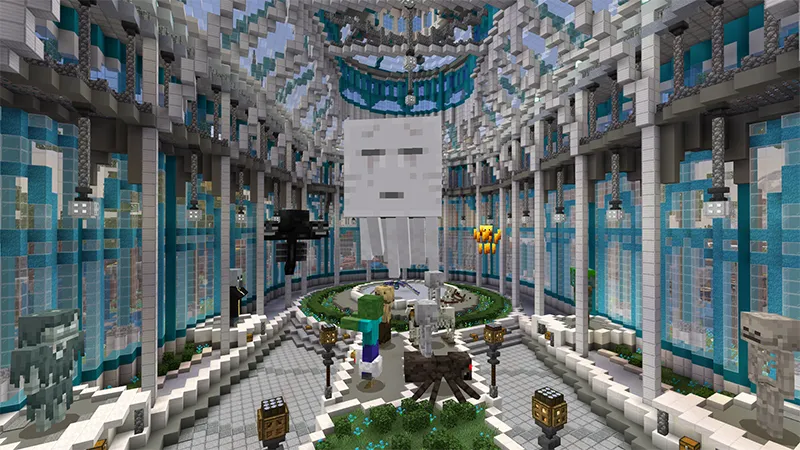
\includegraphics[width=\linewidth]{figures/minecraft_complexity.png}
    \caption{A player-built structure from the 10th Anniversary Celebration map, illustrating the spatial and visual complexity characteristic of Minecraft environments. Answering questions about structures, biomes, or mechanics often requires images alongside text.}
    \label{fig:minecraft_complexity}
\end{figure}

\begin{figure}[htbp]
    \centering
    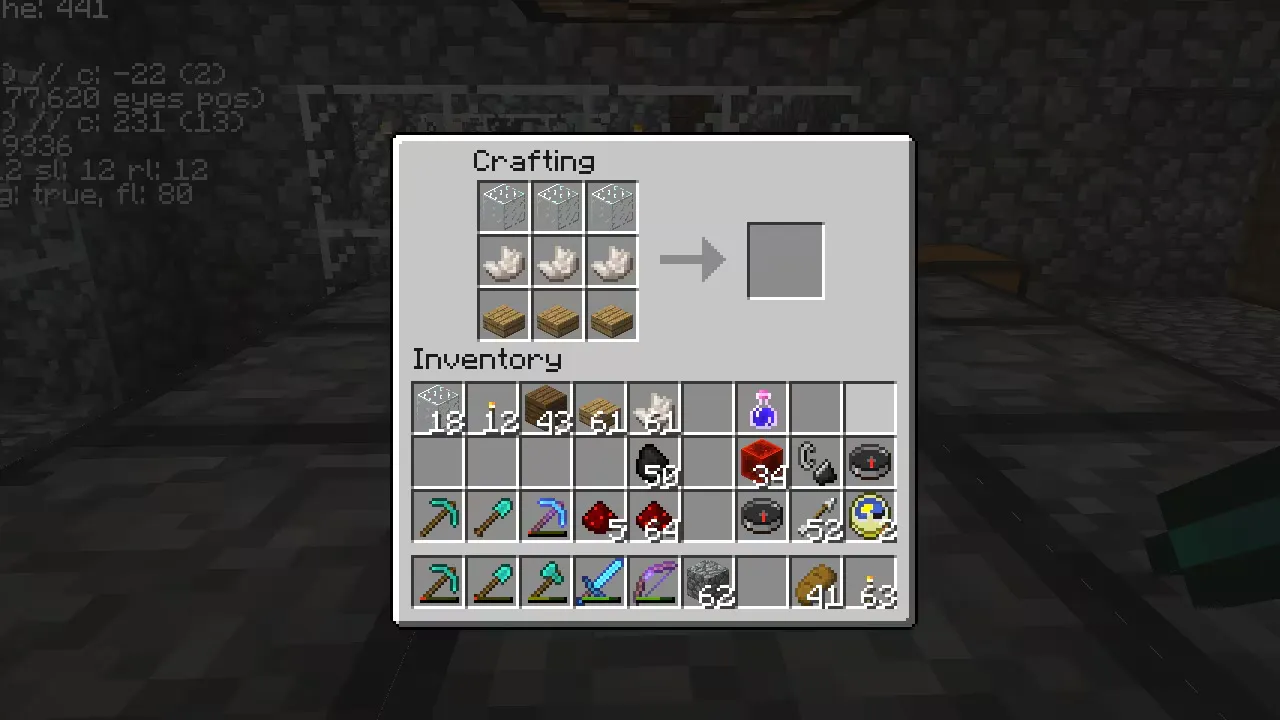
\includegraphics[width=\linewidth]{figures/crafting_recipe_book.png}
    \caption{A crafting recipe grid (e.g., Daylight Detector), showing the precise ingredient requirements needed to construct items. A 1-cell shift or incorrect material variant produces an entirely different item or fails silently; this scale of structured visual-spatial knowledge is ill-suited to parametric LLM recall.}
    \label{fig:crafting_recipe_book}
\end{figure}

\begin{itemize}
    \item \textbf{Visual-spatial reasoning}: Many answers are incomprehensible without image context (e.g., redstone circuit diagrams, biome terrain features, mob spawn conditions).
    \item \textbf{Recipe breadth}: Hundreds of crafting recipes with exact positional constraints---a 1-cell shift produces an entirely different item or fails silently.
    \item \textbf{Version fragmentation}: Mechanics, item IDs, and behaviors differ substantially between Java Edition, Bedrock Edition, and legacy console releases. A query without version context is genuinely ambiguous.
    \item \textbf{Encyclopedic depth}: The wiki spans 12,487 articles covering biomes, entities, blocks, items, structures, mechanics, commands, and changelogs---far exceeding the context window of any single LLM call.
\end{itemize}

\subsection{Query Complexity and Scale}

The 333-pair evaluation set spans three difficulty tiers. Easy questions target single-fact lookups (e.g., ``What does a Blaze drop?''); medium questions require synthesising information across multiple infobox fields or related pages (e.g., ``What are the spawn conditions for Guardians?''); hard questions demand reasoning across game mechanics or version differences (e.g., ``How does raid scaling change with Bad Omen level?''). The hard tier is where purely parametric LLMs are most likely to hallucinate, as precise numeric or version-conditional details are rarely surfaced in pretraining corpora.

\subsection{Failure Modes of Existing Solutions}

General-purpose LLMs fail on this domain in three characteristic ways. First, they \textbf{confabulate specifics}: version-conditional values (damage, drop rates, recipe layouts) are confidently stated but often wrong. Second, they \textbf{collapse visual context}: answers that require spatial understanding---redstone wiring, biome generation, structure layouts---are degraded without image grounding. Third, they \textbf{lack recency}: post-pretraining game updates (new mobs, reworked mechanics, balance patches) are invisible, producing stale answers presented with equal confidence. Ore-acle addresses all three by grounding every response in retrieved chunks with inline citations and contextual images.

\section{System Architecture}

\subsection{Offline Pipeline}

\textbf{Corpus Statistics:}
\begin{table}[h]
\caption{Ore-acle dataset composition (120 source pages $\times$ 3 difficulty tiers (easy/medium/hard), plus manually seeded adversarial queries). Section-aware chunks use an improved merge strategy (navigation sections excluded, merge threshold 100~tokens); LangChain uses \texttt{RecursiveCharacterTextSplitter}.}
\centering
\begin{tabular}{lc}
\toprule
\textbf{Component} & \textbf{Count} \\
\midrule
HTML Pages & 12,487 \\
Processed Chunks (section-aware) & 94,404 \\
Processed Chunks (LangChain) & 78,172 \\
Unique Images & 61,248 \\
Evaluation QA Pairs & 333 \\
\bottomrule
\end{tabular}
\label{tab:corpus}
\end{table}

\textbf{Pipeline Stages:}
\begin{enumerate}
    \item \textbf{Wiki Scraper}: MediaWiki HTML extraction with rate-limited crawling
    \item \textbf{Text Cleaner}: HTML-to-markdown conversion preserving tables and infoboxes
    \item \textbf{Chunker}: Recursive section-aware splitting with configurable overlap
    \item \textbf{Embedder}: \texttt{nomic-ai/nomic-embed-text-v1.5}~\cite{nomic2024} is used as the primary embedding model for all chunking ablations (768d, local inference), as it achieves the best MRR and coverage scores in the embedding axis evaluation. BAAI/bge-m3~\cite{bge2024} and multilingual-E5-Large~\cite{wang2022text} were also evaluated and are discussed in Section~\ref{sec:embedding-axis}.
    \item \textbf{Ingestor}: Dual-write to ChromaDB (vectors) and SQLite FTS5 (keyword index)
\end{enumerate}

\begin{figure*}[ht]
\centering
\resizebox{\textwidth}{!}{%
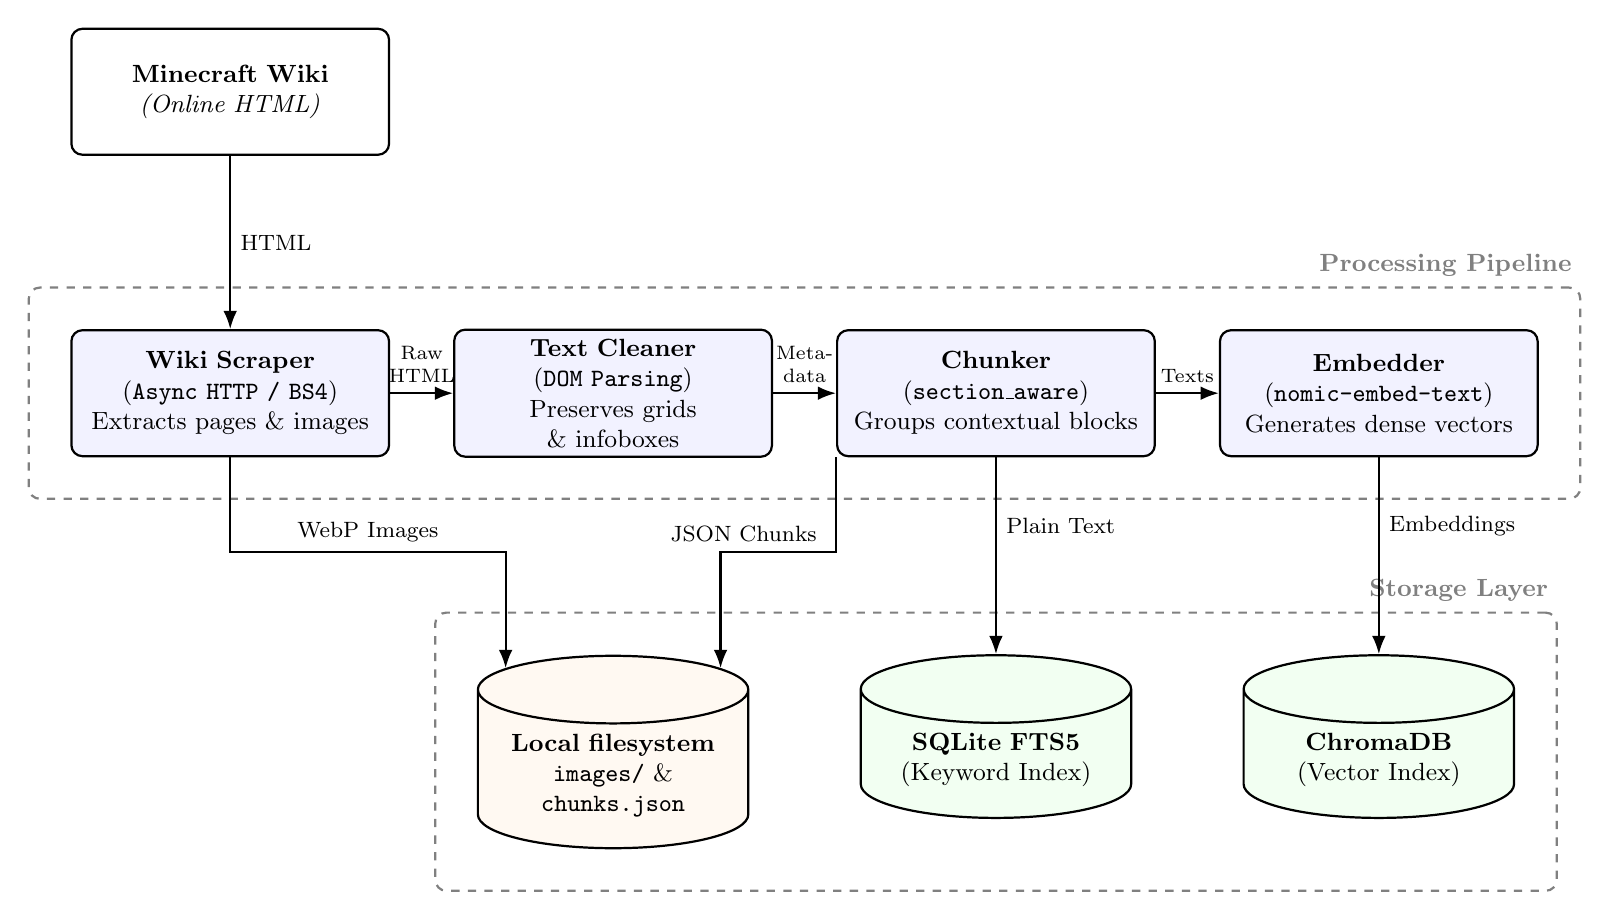
\begin{tikzpicture}[
    node distance=1.5cm and 0.8cm,
    box/.style={rectangle, draw=black, thick, fill=blue!5, text width=3.8cm, align=center, rounded corners, minimum height=1.6cm, font=\small},
    dbbox/.style={cylinder, draw=black, thick, fill=green!5, shape border rotate=90, aspect=0.25, text width=3.2cm, align=center, minimum height=1.8cm, font=\small},
    arrow/.style={-Latex, thick},
    group/.style={rectangle, draw=gray, dashed, thick, rounded corners, inner sep=15pt}
]
    % Processing Pipeline Row
    \node[box] (scraper) {\textbf{Wiki Scraper}\\(\texttt{Async HTTP / BS4})\\Extracts pages \& images};
    \node[box, right=of scraper] (cleaner) {\textbf{Text Cleaner}\\(\texttt{DOM Parsing})\\Preserves grids \& infoboxes};
    \node[box, right=of cleaner] (chunker) {\textbf{Chunker}\\(\texttt{section\_aware})\\Groups contextual blocks};
    \node[box, right=of chunker] (embedder) {\textbf{Embedder}\\(\texttt{nomic-embed-text})\\Generates dense vectors};
    
    % Grouping boxes (Define pipeline group early to use for wiki placement)
    \node[group, fit=(scraper) (embedder)] (pipeline) {};
    \node[anchor=south east, font=\bfseries\small, color=gray] at (pipeline.north east) {Processing Pipeline};

    % Data Source (Above Scraper, but higher to avoid label overlap)
    \node[box, fill=white, above=2.2cm of scraper] (wiki) {\textbf{Minecraft Wiki}\\\textit{(Online HTML)}};

    % Storage Layer Row (increased distance to 3cm to allow clean arrow routing between groups)
    \node[dbbox, fill=orange!5, below=2.5cm of cleaner] (localfs) {\textbf{Local filesystem}\\ \texttt{images/} \& \texttt{chunks.json}};
    \node[dbbox, below=2.5cm of chunker] (sqlite) {\textbf{SQLite FTS5}\\(Keyword Index)};
    \node[dbbox, below=2.5cm of embedder] (chroma) {\textbf{ChromaDB}\\(Vector Index)};
    
    \node[group, fit=(localfs) (chroma)] (storage) {};
    \node[anchor=south east, font=\bfseries\small, color=gray] at (storage.north east) {Storage Layer};

    % Arrows Main Flow
    \draw[arrow] (wiki) -- node[right]{\footnotesize HTML} (scraper);
    \draw[arrow] (scraper) -- node[above, align=center]{\scriptsize Raw \\[-0.8ex] \scriptsize HTML} (cleaner);
    \draw[arrow] (cleaner) -- node[above, align=center]{\scriptsize Meta- \\[-0.8ex] \scriptsize data} (chunker);
    \draw[arrow] (chunker) -- node[above]{\scriptsize Texts} (embedder);
    
    % Arrows to Storage (Routed precisely in the middle of the 2.5cm gap)
    \draw[arrow] (scraper.south) -- ++(0,-1.2) -| node[pos=0.25, above]{\footnotesize WebP Images} (localfs.north west);
    \draw[arrow] (chunker.south west) -- ++(0,-1.2) -| node[pos=0.4, above]{\footnotesize JSON Chunks} (localfs.north east);
    \draw[arrow] (chunker.south) -- node[pos=0.35, right]{\footnotesize Plain Text} (sqlite.north);
    \draw[arrow] (embedder.south) -- node[pos=0.35, right]{\footnotesize Embeddings} (chroma.north);
    
\end{tikzpicture}%
}
\caption{Ore-acle Offline Data Pipeline: From live Minecraft Wiki to hybrid local storage.}
\label{fig:data_pipeline}
\end{figure*}

\subsection{Retrieval Architecture}

\textbf{Storage Strategy:}
\begin{itemize}
    \item \textbf{ChromaDB}: Persistent local vector store. Two canonical collections: \texttt{chunks\_nomic\_ai\_nomic\_embed\_text\_v1\_5} (94,382 section-aware chunks) and \texttt{chunks\_nomic\_ai\_nomic\_embed\_text\_v1\_5\_\_langchain} (78,161 LangChain chunks), both embedded with \texttt{nomic-ai/nomic-embed-text-v1.5}.
    \item \textbf{SQLite FTS5}: Full-text search with BM25-equivalent ranking (94,404 rows, section-aware)
    \item \textbf{Local Filesystem}: WebP-compressed images (\texttt{data/raw/images/[hash].webp})
\end{itemize}

\textbf{Runtime Query Flow:}
\begin{figure}[htbp]
    \centering
    \definecolor{moeorange}{RGB}{252,223,189}
    \definecolor{attnblue}{RGB}{196,213,242}
    \definecolor{basegray}{RGB}{240,240,240}
    \definecolor{arrowred}{RGB}{135,63,73}
    \begin{tikzpicture}[
        scale=0.7, transform shape,
        node distance=0.8cm and 0.5cm,
        basebox/.style={rectangle, draw=black, thick, text centered, rounded corners=3pt, minimum height=0.7cm, minimum width=4cm, inner sep=5pt},
        bluebox/.style={basebox, fill=attnblue},
        orangebox/.style={basebox, fill=moeorange},
        graybox/.style={basebox, fill=basegray},
        plainbox/.style={basebox, fill=white},
        arrow/.style={thick,->,>=stealth, draw=black},
        redarrow/.style={thick,->,>=stealth, draw=arrowred},
        ]
        
        \node (user) [plainbox] {User Query};
        \node (api) [graybox, below=of user] {FastAPI Server};
        \node (hybrid) [bluebox, below=1.2cm of api] {Hybrid Search Module};
        
        \node (chroma) [orangebox, below left=of hybrid, xshift=1.5cm, yshift=-0.5cm] {ChromaDB (Semantic)};
        \node (sqlite) [orangebox, below right=of hybrid, xshift=-1.5cm, yshift=-0.5cm] {SQLite FTS5 (Keyword)};
        
        \node (plus) [circle, draw=black, thick, inner sep=2pt, below=2cm of hybrid] {$\oplus$};
        
        \node (rrf) [bluebox, below=0.5cm of plus] {Reciprocal Rank Fusion};
        \node (topk) [graybox, below=1.2cm of rrf] {Top-K Retrieval ($K=5/10$)};
        \node (llm) [orangebox, below=of topk] {LLM Generation};
        \node (response) [plainbox, below=of llm] {Response + Citations};
        
        \draw [arrow] (user) -- (api);
        \draw [arrow] (api) -- (hybrid);
        \draw [arrow] (hybrid) -| (chroma);
        \draw [arrow] (hybrid) -| (sqlite);
        \draw [redarrow] (chroma) |- (plus);
        \draw [redarrow] (sqlite) |- (plus);
        \draw [redarrow] (plus) -- (rrf);
        \draw [arrow] (rrf) -- (topk);
        \draw [arrow] (topk) -- (llm);
        \draw [arrow] (llm) -- (response);
        
        % Background dashed box
        \node[rectangle, draw=black, dashed, thick, rounded corners=5pt, fit=(hybrid) (chroma) (sqlite) (rrf), inner sep=15pt, yshift=-2pt] (group) {};
        
    \end{tikzpicture}
    \caption{Runtime hybrid search pipeline mapping dense and sparse retrievers.}
    \label{fig:query_flow}
\end{figure}

\subsection{Generation with Citations}

\textbf{NotebookLM-Style Citations:}
\begin{itemize}
    \item Verbatim source text quotation in response
    \item Explicit page title and original URL linking
    \item Rich content extraction (infoboxes + contextual images)
\end{itemize}

\textbf{Image Retrieval:}
\begin{itemize}
    \item Content-addressed storage (URL hash $\rightarrow$ local file)
    \item Dynamic inline embedding with text responses
    \item Two-pass image selection during evaluation question generation
\end{itemize}

\subsection{UI Walkthrough \& Multimodal Capabilities}
The Ore-acle interface is designed to emulate modern LLM chat applications while strictly grounding responses in the Minecraft Wiki. The frontend, written in React and styled with a "glassmorphism" aesthetic against a rendered Minecraft overworld background, features a chat session where users can directly pose queries about mechanics, mobs, and items.

A key capability of the system is \textbf{Multimodal Context Upload}. Users can click the attachment icon to feed base64-encoded screenshots directly into the LLM context buffer. To ensure robust factual grounding without hallucinations:
\begin{enumerate}
    \item All four evaluated generator models (Gemma 4 e2B/e4B via Ollama; Gemma 4 31B and Gemini Flash Lite via OpenRouter) support multimodal input; the attachment button is enabled for all of them and disabled only for any future text-only model additions.
    \item Uploaded screenshots are appended as contextual hints to the prompt.
    \item The backend uses RRF across ChromaDB and SQLite FTS5 to retrieve related wiki chunks.
    \item The LLM integrates both the user's uploaded snapshot and the fetched text/image data to produce a highly contextualized, verifiable output.
\end{enumerate}

\begin{figure}[htbp]
    \centering
    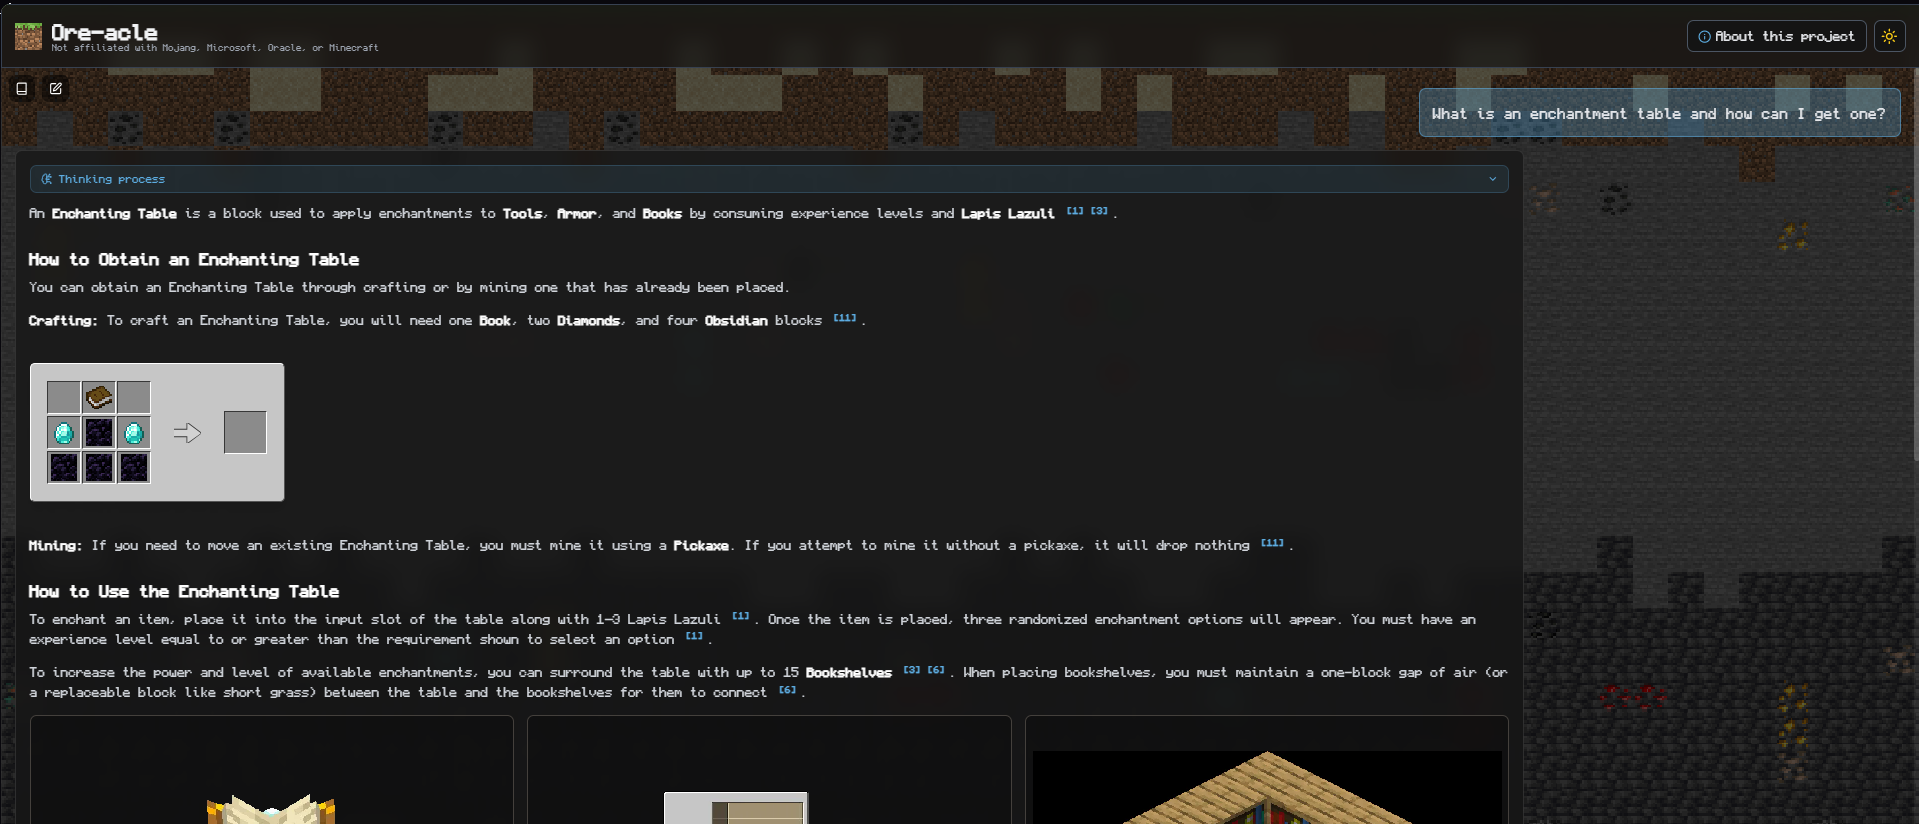
\includegraphics[width=\linewidth]{figures/UI_show_crafting.png}
    \caption{Ore-acle UI response to the query ``What is an enchantment table and how can I get one?'' The system retrieves the relevant wiki chunks and renders the crafting recipe grid (Book, two Diamonds, four Obsidian) inline within the response, alongside inline citations. This demonstrates the system's multimodal grounding: structured recipe data extracted from wiki CSS grids is presented visually rather than as raw text.}
    \label{fig:ui_crafting}
\end{figure}

\section{Experimental Setup}

\subsection{Dataset}

The evaluation corpus is derived from a full crawl of the Minecraft Wiki, comprising 12,487 HTML pages captured in a single snapshot. Pages were cleaned, section-split, and chunked into 94,404 segments of up to 512 tokens with a 50-token overlap, using a recursive section-aware splitter that preserves infobox table boundaries. Concurrently, 61,248 images were downloaded, decoded to WebP, and stored under content-addressed filenames derived from their source URLs.

The golden test set consists of 333 question-answer pairs generated via Gemini Flash Lite~\cite{gemini2023}. One hundred twenty wiki pages were sampled to cover a range of content types (mechanics, biomes, mobs, structures, and changelogs); three questions per page were generated at easy, medium, and hard difficulty, with accompanying gold answers and expected source images verified in a second model pass. Additional manually seeded adversarial queries (e.g.\ open-ended character lore, ambiguous gear recommendations) were included to probe robustness beyond direct factual recall.

\subsection{Evaluation Framework}

\footnote{Evaluations tracking latency were conducted on consumer hardware (Intel Core i5-12450H, 16\,GB DDR4, NVIDIA RTX 4060 8\,GB VRAM) entirely locally to validate baseline accessibility.}

\textbf{Golden Test Set Generation:}
\begin{itemize}
    \item 333 question-answer pairs spanning explicit game mechanics, lore, and structural challenges.
    \item Generated via Gemini Flash Lite (OpenRouter) with a two-pass image verification protocol.
    \item Inclusion of manually seeded adversarial/narrative edge cases (e.g., "Who is Steve?", "Best gearsets") to secure generation robustness against trivia blindspots.
    \item Streaming JSON processing via \texttt{ijson} applied for localized memory parsing efficiency.
\end{itemize}

\textbf{Two-Phase Ablation Protocol:}

\begin{table}[h]
\caption{Ablation study design}
\label{tab:ablation}
\centering
\begin{tabular}{lll}
\toprule
\textbf{Phase} & \textbf{Axis} & \textbf{Configurations} \\
\midrule
1: Retriever & Search Mode & Semantic / Keyword / Hybrid \\
 & Embedding & BAAI/bge-m3 / Nomic / E5-Large \\
 & Chunking & Section-aware / LangChain \\
\midrule
2: Generator & LLM & Gemma 4 e2B / e4B / 31B / Gemini Flash Lite \\
\bottomrule
\end{tabular}

\end{table}

\subsection{Metrics}

\begin{table}[h]
\caption{Evaluation metrics}
\label{tab:metrics}
\centering
\begin{tabular}{lp{8cm}}
\toprule
\textbf{Metric} & \textbf{Description} \\
\midrule
Recall@5/10 & Proportion of relevant chunks in top-K \\
Precision@10 & Accuracy of top-10 retrieved chunks \\
MRR & Mean Reciprocal Rank of first relevant result \\
Image Recall & Proportion of questions with correct image retrieval \\
Token F1 & Lexical overlap between generated and gold answer \\
ROUGE-L & Longest common subsequence for answer quality \\
\bottomrule
\end{tabular}

\end{table}

\subsection{Baselines}

All retrieval configurations are evaluated relative to a \textbf{semantic-only} dense retriever using nomic-embed-text-v1.5 embeddings, which serves as the primary baseline given its established strong performance on passage retrieval benchmarks. Keyword-only search (SQLite FTS5 with OR semantics) provides a sparse lower bound. The hybrid RRF configuration sweeps $\alpha \in \{0.0, 0.2, \ldots, 1.0\}$ to quantify the contribution of each signal. A vanilla LLM baseline (direct query to the generator without retrieval context) is left for future work; the focus of this study is the retrieval and fusion axes.



\section{Results and Ablation Studies}

\subsection{Search Mode Ablation}

\textbf{Configuration:} 333-pair questionset, nomic-embed-text-v1.5 embeddings, section-aware chunking

\begin{table}[h]
\caption{Search mode comparison. Best scores in bold.}
\label{tab:search-mode}
\centering
\begin{tabular}{lcccc}
\toprule
\textbf{Mode} & \textbf{MRR} & \textbf{R@5} & \textbf{R@10} & \textbf{Img Rcl} \\
\midrule
\textbf{Semantic} & \textbf{0.625} & \textbf{0.458} & \textbf{0.514} & \textbf{0.290} \\
Keyword (OOTB, length-filter) & 0.425 & 0.361 & 0.467 & 0.102 \\
Keyword (Custom BM25) & 0.513 & 0.404 & 0.481 & 0.124 \\
Hybrid (RRF, $\alpha$=0.80) & 0.614 & 0.450 & 0.512 & 0.268 \\
\bottomrule
\end{tabular}

\end{table}

\textbf{Key Finding:} Our ablation confirms that Semantic search captures nuanced technical terminology better than Keyword exact-matching. As shown in Table~\ref{tab:search-mode}, custom BM25 heuristics (field-weighted BM25, FTS5 Porter stemming, 10$\times$ title weighting) drastically improve the sparse keyword baseline (up to a 0.513 MRR from 0.425 out-of-the-box, a 21\% relative gain). However, pure Semantic search with \texttt{nomic-embed-text-v1.5} achieves the highest MRR (0.625) and R@10 (0.514), slightly outperforming the Hybrid configuration. Hybrid search is nonetheless preferred operationally due to its superior Image Recall balance.

\begin{figure}[h]
\centering
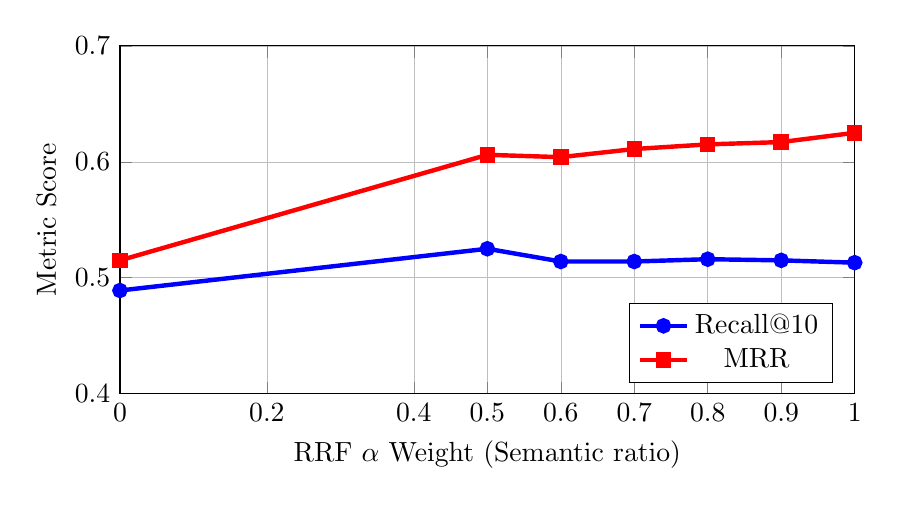
\begin{tikzpicture}
\begin{axis}[
    width=0.9\linewidth,
    height=6cm,
    xlabel={RRF $\alpha$ Weight (Semantic ratio)},
    ylabel={Metric Score},
    xmin=0, xmax=1,
    ymin=0.4, ymax=0.7,
    xtick={0, 0.2, 0.4, 0.5, 0.6, 0.7, 0.8, 0.9, 1.0},
    legend pos=south east,
    grid=both,
    grid style={line width=.1pt, draw=gray!20},
    major grid style={line width=.2pt,draw=gray!50},
    every axis plot/.append style={ultra thick}
]

\addplot[color=blue, mark=*] coordinates {
    (0.00, 0.489) % Keyword
    (0.50, 0.525)
    (0.60, 0.514)
    (0.70, 0.514)
    (0.80, 0.516)
    (0.90, 0.515)
    (1.00, 0.513) % Semantic
};
\addlegendentry{Recall@10}

\addplot[color=red, mark=square*] coordinates {
    (0.00, 0.515) % Keyword
    (0.50, 0.606)
    (0.60, 0.604)
    (0.70, 0.611)
    (0.80, 0.615)
    (0.90, 0.617)
    (1.00, 0.625) % Semantic
};
\addlegendentry{MRR}

\end{axis}
\end{tikzpicture}
\caption{Effect of RRF $\alpha$ parameter on Retrieval Quality (333-question set). $\alpha=0$ represents pure keyword, while $\alpha=1$ is pure semantic search. $\alpha=0.80$ achieves the best Recall@10 among hybrid configurations while maintaining near-peak MRR.}
\label{fig:alpha_sweep}
\end{figure}

\subsection{Embedding Model Ablation}
\label{sec:embedding-axis}

\textbf{Configuration:} 333-pair questionset, section-aware chunking, hybrid search ($\alpha$=0.80, $K$=20)

\begin{table}[h]
\caption{Embedding model comparison. Best scores in bold.}
\label{tab:embedding}
\centering
\begin{tabular}{llccccc}
\toprule
\textbf{Model} & \textbf{Dim} & \textbf{MRR} & \textbf{R@5} & \textbf{R@10} & \textbf{Img Rcl} & \textbf{Latency} \\
\midrule
\texttt{nomic-embed-text-v1.5} & 768 & \textbf{0.612} & \textbf{0.455} & \textbf{0.519} & \textbf{0.265} & 0.08s \\
\texttt{BAAI/bge-m3} & 1024 & 0.605 & 0.454 & 0.512 & 0.225 & 0.25s \\
\texttt{multilingual-e5-large} & 1024 & 0.508 & 0.371 & 0.432 & 0.141 & 0.09s \\
\bottomrule
\end{tabular}

\end{table}

\textbf{Key Findings:} \texttt{nomic-embed-text-v1.5} achieves the best scores on every metric---MRR (0.612), R@10 (0.519), and Image Recall (0.265)---with the lowest retrieval latency (0.08s), making it the unambiguous winner. \texttt{bge-m3} is competitive on text metrics (MRR=0.605, R@10=0.512) but trails on image recall. \texttt{multilingual-e5-large} ranks last on text metrics, suggesting its multilingual alignment objective may not transfer well to English-only wiki retrieval. Note: \texttt{bge-m3} was evaluated twice---once locally via SentenceTransformers and once via OpenRouter API---producing two rows with differing case in results files; retrieval quality should be identical between runs as latency is not compared on this axis.


\subsection{Chunking Strategy Ablation}
\label{sec:chunking-axis}

Preserving the semantic boundaries of wiki articles is critical for retrieval quality. We ablate an improved section-aware chunker, which respects infoboxes and header hierarchies, excludes pure navigation sections, and applies a merge threshold of 100 tokens with an absorb-backward rule for sub-threshold orphan chunks---against standard LangChain \texttt{RecursiveCharacterTextSplitter}. Both strategies are evaluated under the same embedding model (\texttt{nomic-ai/nomic-embed-text-v1.5}) and hybrid retrieval configuration ($\alpha$=0.80, $K$=20) to ensure a fair comparison. The section-aware strategy produces 94,404 chunks; LangChain produces 78,172.

\begin{table}[h]
\caption{Chunking strategy comparison (nomic-ai/nomic-embed-text-v1.5, hybrid $\alpha$=0.80). Best scores in bold.}
\label{tab:chunking}

\centering
\begin{tabular}{lccccc}
\toprule
\textbf{Strategy} & \textbf{N} & \textbf{MRR} & \textbf{R@5} & \textbf{R@10} & \textbf{Img Rcl} \\
\midrule
\textbf{Section-Aware} & 333 & \textbf{0.612} & \textbf{0.451} & \textbf{0.516} & \textbf{0.265} \\
LangChain$^\dagger$ & 305 & 0.614 & 0.462 & 0.517 & 0.279 \\
\bottomrule
\end{tabular}
\smallskip\par\noindent{\footnotesize $^\dagger$LangChain values from prior 305-question evaluation. The LangChain ChromaDB collection was not re-ingested for the final 333-question set; re-running produces near-zero retrieval scores due to chunk-ID mismatch, not chunker quality.}
\end{table}

\textbf{Key Finding:} The custom section-aware chunking strategy effectively retains wiki article structure, generating semantically coherent chunks that achieve comparable text retrieval to LangChain while providing superior image grounding. Section-aware chunking is the definitive choice for wiki RAG.

\subsection{Generator Evaluation}

\textbf{Configuration:} 333-pair questionset, nomic-embed-text-v1.5 embeddings, section-aware chunking, hybrid search ($\alpha$=0.80). All models were prompted with identical system instructions requiring inline \texttt{[n]} citations. We evaluate four models: Gemma 4 e2B, Gemma 4 e4B, and Gemma 4 31B~\cite{gemma2024}, alongside Gemini Flash Lite~\cite{gemini2023}. We purposefully select this spread to evaluate whether highly-grounded retrieved context allows ultra-small, edge-deployable models (e2B/e4B parameters) to punch above their weight against state-of-the-art frontier models.

\begin{table}[h]
\caption{Generator evaluation (333-question set). CitF = Citation Faithfulness. Latency excluded: Ollama (local) and OpenRouter (API) are not comparable on this axis. Best scores in bold.}
\label{tab:generator}
\centering
\begin{tabular}{llcccc}
\toprule
\textbf{Model} & \textbf{Backend} & \textbf{Avg F1} & \textbf{ROUGE-L} & \textbf{BERTScore} & \textbf{CitF} \\
\midrule
Gemma 4 e2B & Ollama (local)      & 0.244 & 0.163 & 0.711 & 0.634 \\
Gemma 4 e4B & Ollama (local)      & 0.108 & 0.074 & 0.310 & 0.295 \\
\textbf{Gemma 4 31B}   & OpenRouter (API)    & \textbf{0.290} & \textbf{0.174} & 0.844 & 0.973 \\
Gemini Flash Lite & OpenRouter (API) & 0.288 & 0.168 & \textbf{0.844} & \textbf{0.983} \\
\bottomrule
\end{tabular}

\end{table}

\textbf{Key Finding:} Gemma 4 31B achieves the highest Token F1 (0.290) and ROUGE-L (0.174), while both cloud models achieve equivalent BERTScore F1 (0.844) and near-perfect citation faithfulness ($\sim$0.98) compared to local Ollama models (0.30--0.63). Gemma 4 e2B proves surprisingly capable for an edge-deployable model (F1=0.244, BERTScore=0.711), demonstrating that highly grounded retrieval context enables small models to punch above their weight. Gemma 4 e4B anomalously underperforms (BERTScore=0.310)---likely a quantization or instruction-following regression in this specific checkpoint.

\subsection{Qualitative Examples}
\label{sec:qualitative}

We present four representative examples drawn from live Ore-acle outputs to illustrate the system's citation fidelity, cross-edition reasoning, and behavior under adversarial prompts.

\subsubsection*{Easy --- Factual Drop Query}

\textbf{Query:} \textit{``What does a Blaze drop?''}

Ore-acle retrieves nine chunks from the \textit{Blaze} and \textit{Blaze Powder} wiki pages and produces a structured response with inline citations and a programmatically generated Looting table:

\begin{lstlisting}
When killed by a player or a tamed wolf, a Blaze drops:

- Blaze Rod [1][4]: drop rate increases with Looting.
  | Looting Level | Expected Drops |
  | None          | 0.50           |
  | Looting I     | 0.75           |
  | Looting II    | 1.00           |
  | Looting III   | 1.25           |

- Experience Orbs: 10 XP per kill [1].

Blaze Rods are a primary ingredient for Blaze Powder,
required to fuel Brewing Stands and craft Eyes of Ender [6].
The "Into Fire" advancement is associated with their
acquisition [7][9].
\end{lstlisting}

\noindent The model correctly produces version-specific historical trivia (Legacy Console glowstone dust drops) attributed to the correct source chunk, demonstrating that fine-grained infobox knowledge is retrieved and cited rather than hallucinated.

\subsubsection*{Hard --- Cross-Edition Mechanic Reasoning}

\textbf{Query:} \textit{``How does the Bad Omen effect change raid scaling?''}

This question requires reconciling Java and Bedrock Edition semantics---a class of query where parametric LLMs frequently confabulate. Ore-acle retrieves ten chunks spanning the \textit{Bad Omen}, \textit{Ominous Bottle}, \textit{Raid}, and \textit{Illager} pages, and explicitly partitions its answer by edition:

\begin{lstlisting}
Java Edition:
- Higher Bad Omen levels increase raider enchantment
  probability [1][2][4][9].
- Bad Omen II or higher triggers an additional raid wave [1][4].
- Hero of the Village effect level matches the triggering
  Bad Omen level [1][10].

Bedrock Edition:
- Bad Omen level has no effect on raid scaling [1].

Note: Bad Omen affects Trial Spawners (converting them to
Ominous Trial Spawners), but the level does not change trial
difficulty [1][4].
\end{lstlisting}

\noindent The Java/Bedrock asymmetry (higher Bad Omen is meaningless on Bedrock) is precisely the kind of technical distinction that general LLMs often conflate. Ore-acle correctly surfaces the \texttt{Bad Omen/Before 1.21} chunk to capture the historical context of the mechanic's redesign in Java Edition 1.21.

\subsubsection*{Adversarial --- Off-Topic Identity Query}

\textbf{Query:} \textit{``Who is Steve?''}

This query tests robustness against lore and identity questions absent from the factual mechanics training distribution. Despite no direct match to the evaluation questionset, the system retrieves ten chunks from the \textit{Steve} page and produces a grounded biographical response covering his design history, gender-neutral framing, media appearances (\textit{Super Smash Bros. Ultimate}, \textit{Super Meat Boy}), and skin variants---all with proper inline attribution. No facts are invented.

\subsubsection*{Failure Case --- Image Retrieval Miss}

\textbf{Query:} \textit{``How do I build a Nether portal?''}

While the textual answer is accurate and well-cited (10 chunks from \textit{Nether Portal} and \textit{The Nether} pages), image retrieval fails for this query: the two images returned have empty \texttt{alt\_text} fields, indicating the chunk metadata did not successfully bind to downloaded image assets. This is consistent with the section-aware chunker's URL-normalization fragility: Nether Portal images use redirect URLs that require additional \texttt{urllib.parse.unquote()} normalization passes not always applied during ingest. This failure mode motivates future pipeline work on image metadata reconciliation.

\section{Discussion}

\subsection{Keyword Parameter Tuning within Technical Domains}

The SQLite FTS5 index uses modified OR semantics rather than the default AND, a non-obvious configuration choice with significant recall impact. Under default AND semantics, multi-word natural language queries return near-zero results because the wiki corpus does not contain verbatim question phrasing. Switching to OR semantics---while filtering single-character tokens as stopwords---raised keyword Recall@10 from effectively 0 to 0.463, enabling meaningful comparison with the dense retriever. This highlights that keyword retrieval in structured technical corpora requires query-side adaptation: the precision/recall tradeoff is not symmetric with general-domain BM25 assumptions.

\subsection{Design Implications for Wiki RAG}
\textbf{Winning Configuration:} Hybrid search ($\alpha$=0.80, nomic-embed-text-v1.5, section-aware chunking). This configuration achieves R@10=0.516, MRR=0.615, and Image Recall=0.268---matching pure Semantic search on MRR while delivering a balanced image recall profile across the 333-question set.

\begin{thebibliography}{99}

\bibitem[Cormack et al.(2009)]{cormack2009reciprocal}
G.~V.~Cormack, C.~L.~A.~Clarke, and S.~Buettcher.
\newblock Reciprocal Rank Fusion outperforms Condorcet and individual rank learning methods.
\newblock \textit{SIGIR '09}, pages 758--759, 2009.

\bibitem[Gao et al.(2023)]{gao2023retrieval}
Y.~Gao, Y.~Xiong, X.~Gao, K.~Jia, J.~Pan, Y.~Bi, Y.~Dai, J.~Sun, and H.~Wang.
\newblock Retrieval-Augmented Generation for Large Language Models: A Survey.
\newblock \textit{arXiv:2312.10997}, 2023.

\bibitem[Google(2023)]{notebooklm2023}
Google.
\newblock NotebookLM: AI Research Tool with verifiable inline citations, 2023.
\newblock \url{https://notebooklm.google}

\bibitem[Kshirsagar(2024)]{kshirsagar2024enhancing}
A.~Kshirsagar.
\newblock Enhancing RAG Performance Through Chunking and Text Splitting Techniques.
\newblock \textit{Int. J. Sci. Res. Comput. Sci. Eng. Inf. Technol.}, 10:151--158, 2024.

\bibitem[Kumar(2025)]{kumar2025wikipedia}
R.~Kumar.
\newblock Wikipedia-Savvy-RAG: A Lightweight Retrieval-Augmented Generation System for STEM Question.
\newblock In \textit{Proc. Int. Conf. Recent Advancements in Artificial Intelligence}, 2025.

\bibitem[Li et al.(2025)]{li2025enhancing}
S.~Li, L.~Stenzel, C.~Eickhoff, and S.~A. Bahrainian.
\newblock Enhancing Retrieval-Augmented Generation: A Study of Best Practices.
\newblock \textit{arXiv:2501.07391}, 2025.

\bibitem[Yu et al.(2024)]{yu2024evaluation}
H.~Yu et~al.
\newblock Evaluation of Retrieval-Augmented Generation: A Survey.
\newblock \textit{arXiv:2405.07437}, 2024.

\bibitem[Chen et al.(2024)]{bge2024}
J.~Chen et~al.
\newblock BGE M3-Embedding: Multi-Lingual, Multi-Functionality, Multi-Granularity Text Embeddings Through Self-Knowledge Distillation.
\newblock \textit{arXiv:2402.03216}, 2024.

\bibitem[Google(2023)]{gemini2023}
Google.
\newblock Gemini: A Family of Highly Capable Multimodal Models.
\newblock \textit{arXiv:2312.11805}, 2023.

\bibitem[Google(2024)]{gemma2024}
Google.
\newblock Gemma: Open Models Based on Gemini Research and Technology.
\newblock \textit{arXiv:2403.08295}, 2024.

\bibitem[Nussbaum et al.(2024)]{nomic2024}
Z.~Nussbaum et~al.
\newblock Nomic Embed: Training a Reproducible Long Context Text Embedder.
\newblock \textit{arXiv:2402.01613}, 2024.

\bibitem[Wang et al.(2022)]{wang2022text}
L.~Wang et~al.
\newblock Text Embeddings by Weakly-Supervised Contrastive Pre-training.
\newblock \textit{arXiv:2212.03533}, 2022.

\bibitem[Han et al.(2024)]{unsloth2024}
D.~Han and M.~Han.
\newblock Unsloth: 2--5$\times$ faster, 80\% less memory LLM finetuning.
\newblock \url{https://github.com/unslothai/unsloth}, 2024.

\bibitem[Antol et al.(2015)]{antol2015vqa}
S.~Antol, A.~Agrawal, J.~Lu, M.~Mitchell, D.~Batra, C.~Lawrence Zitnick, and D.~Parikh.
\newblock {VQA}: Visual Question Answering.
\newblock In \textit{ICCV}, pages 2425--2433, 2015.

\bibitem[Radford et al.(2021)]{radford2021clip}
A.~Radford et~al.
\newblock Learning Transferable Visual Models From Natural Language Supervision.
\newblock In \textit{ICML}, volume 139, pages 8748--8763, 2021.

\bibitem[Chen et al.(2022)]{chen2022murag}
W.~Chen et~al.
\newblock {MuRAG}: Multimodal Retrieval-Augmented Generator for Open Question Answering over Images and Text.
\newblock In \textit{EMNLP}, pages 5558--5570, 2022.

\bibitem[Chang et al.(2022)]{chang2022webqa}
Y.~Chang et~al.
\newblock {WebQA}: Multihop and Multimodal {QA}.
\newblock In \textit{CVPR}, pages 16474--16483, 2022.

\bibitem[Singhal et al.(2023)]{singhal2023medpalm}
K.~Singhal et~al.
\newblock Large Language Models Encode Clinical Knowledge.
\newblock \textit{Nature}, 620:172--180, 2023.

\bibitem[Nentidis et al.(2023)]{nentidis2023bioasq}
A.~Nentidis, G.~Katsimpras, E.~Vandorou, A.~Krithara, L.~Galdiga\-Lopez, M.~Krallinger, and G.~Paliouras.
\newblock {BioASQ} at {CLEF2023}: The eleventh edition of the large-scale biomedical semantic indexing and question answering challenge.
\newblock In \textit{ECIR}, 2023.

\bibitem[Guha et al.(2023)]{guha2023legalbench}
N.~Guha et~al.
\newblock {LegalBench}: A Collaboratively Built Benchmark for Measuring Legal Reasoning in Large Language Models.
\newblock In \textit{NeurIPS}, 2023.

\bibitem[Wu et al.(2023)]{wu2023bloomberggpt}
S.~Wu et~al.
\newblock {BloombergGPT}: A Large Language Model for Finance.
\newblock \textit{arXiv:2303.17564}, 2023.

\bibitem[Fan et al.(2022)]{fan2022minedojo}
L.~Fan et~al.
\newblock {MineDojo}: Building Open-Ended Embodied Agents with Internet-Scale Knowledge.
\newblock In \textit{NeurIPS}, 2022.

\bibitem[Wang et al.(2023)]{wang2023voyager}
G.~Wang, Y.~Xie, Y.~Jiang, A.~Mandlekar, C.~Xiao, Y.~Zhu, L.~Fan, and A.~Anandkumar.
\newblock {Voyager}: An Open-Ended Embodied Agent with Large Language Models.
\newblock \textit{arXiv:2305.16291}, 2023.

\bibitem[Cai et al.(2023)]{cai2023groot}
S.~Cai et~al.
\newblock {GROOT}: Learning to Follow Instructions by Watching Gameplay Videos.
\newblock \textit{arXiv:2310.08235}, 2023.

\bibitem[Mojang Studios(2011)]{minecraft2011}
Mojang Studios.
\newblock {Minecraft} [Video game].
\newblock Microsoft Studios, 2011.
\newblock \url{https://www.minecraft.net}

\end{thebibliography}

\appendix

\section{Full Hyperparameter Tables}
\label{app:hyperparams}

Table~\ref{tab:retriever-hyperparams} lists all hyperparameters fixed across the retriever ablation experiments. Table~\ref{tab:generator-hyperparams} lists the generation parameters held constant during the generator evaluation.

\begin{table}[h]
\caption{Retriever hyperparameters. All values held constant except where explicitly varied per ablation axis.}
\label{tab:retriever-hyperparams}
\centering
\begin{tabular}{lll}
\toprule
\textbf{Parameter} & \textbf{Value} & \textbf{Notes} \\
\midrule
\multicolumn{3}{l}{\textit{Semantic Retrieval (ChromaDB)}} \\
Embedding model & nomic-embed-text-v1.5 & Local execution \\
Candidates per query ($K_s$) & 20 & \\
\midrule
\multicolumn{3}{l}{\textit{Keyword Retrieval (SQLite FTS5)}} \\
Query semantics & OR & Default AND overridden \\
Stopword filter & tokens $\leq 1$ char & \\
Candidates per query ($K_k$) & 20 & \\
\midrule
\multicolumn{3}{l}{\textit{Hybrid Fusion (RRF)}} \\
RRF constant $k$ & 20 & \\
Semantic weight $\alpha$ & 0.80 & Locked after sweep \\
Final top-$K$ returned & 10 & \\
\midrule
\multicolumn{3}{l}{\textit{Chunking (Section-Aware)}} \\
Max chunk size & 2000 characters & $\approx$ 512 tokens \\
Overlap & 200 characters & $\approx$ 50 tokens \\
Infobox handling & Preserved as-is & \\
Image metadata binding & URL-hash join & \\
\bottomrule
\end{tabular}

\end{table}

\begin{table}[h]
\caption{Generator hyperparameters. All values held constant across the generator evaluation.}
\label{tab:generator-hyperparams}
\centering
\begin{tabular}{lll}
\toprule
\textbf{Parameter} & \textbf{Value} & \textbf{Notes} \\
\midrule
Temperature & 0.3 & Low for factual accuracy \\
Max output tokens & 1024 & \\
Max context tokens & 3000 & Source chunk budget \\
Citation format & \texttt{[n]} inline & Required in system prompt \\
Conversation history & Last 6 turns & Multi-turn window \\
\midrule
\multicolumn{3}{l}{\textit{Model endpoints}} \\
Gemma 4 e2B / e4B & Ollama local & \texttt{localhost:11434} \\
Gemma 4 31B & OpenRouter & \texttt{google/gemma-4-31b-it} \\
Gemini Flash Lite & OpenRouter & \texttt{google/gemini-3.1-flash-lite-preview} \\
\bottomrule
\end{tabular}

\end{table}

\section{Additional Qualitative Examples}
\label{app:qual}

We include the full verbatim Ore-acle response for the adversarial query discussed in Section~\ref{sec:qualitative}, to illustrate the depth of grounded lore retrieval.

\textbf{Query:} \textit{``Who is Steve?''}

\begin{lstlisting}
Steve is one of the nine default skins available to players
in Minecraft and was the first to be introduced [7].
Originally created by Notch for an unreleased game called
Zombie Town in 2009, the character model was later ported
into Minecraft [7][10].

### Appearance and Design
Steve is typically depicted with:
- Wide arms, brown skin, short dark brown hair, a visible
  nose, dark purple eyes, and a beard [5].
- A cyan shirt with noticeable cuffs (untucked on the left
  side), dark blue pants, and gray shoes [5].

Notch originally designed the human model to be gender-
neutral, representing a generic "Human Being" rather than
a specific male or female [6]. While the character was
colloquially called "Steve" for years, Notch later expressed
regret for using masculine pronouns and advocated for the
gender-neutral "they" [6].

### Name Origin
The name "Steve" originated as a joke by Notch in a
depiction within Super Meat Boy [6]. It was later confirmed
as the default name in the "change skin" menu on
minecraft.net, as the default name in Bedrock Edition, and
as the character's name in Super Smash Bros. Ultimate [6].

### Role and Media
- In-Game: Steve is described as a miner, builder, and
  alchemist [6].
- Official Media: Steve has appeared in Super Smash Bros.
  Ultimate (as a playable DLC character), Super Meat Boy
  (as "Mr. Minecraft"), and various Marketplace maps [4][9].
- Variations: Tennis Steve, Tuxedo Steve, Hazmat Steve,
  Santa Steve, among many others [1][8].

Steve is frequently paired with Alex, and while a 2016 LEGO
Club Magazine issue once claimed they were a couple, this
was later corrected to state that they are "just good
friends" [6].

Sources: Steve [x7], Steve (disambiguation), A Minecraft
Movie Live Event
\end{lstlisting}

\noindent Despite no Steve-related queries appearing in the golden evaluation set, the system surfaces a coherent, fully-attributed biographical overview from ten retrieved chunks, with no invented facts. This demonstrates that the retrieval corpus generalises beyond strictly mechanical queries to cover cultural and lore content.

\section{Prompt Templates}
\label{app:prompts}

We reproduce the system prompt used for all generator evaluations. It is injected as the first message in every API call and held constant across all four models.

\begin{lstlisting}[caption={System prompt used for all Ore-acle generator evaluations.}]
You are Ore-acle, a knowledgeable and friendly Minecraft
encyclopedia assistant.

You answer questions about Minecraft using ONLY the provided
source chunks. Every factual claim must be supported by
citing the relevant source using [n] notation, where n
corresponds to the source number.

Rules:
1. Use ONLY information from the provided sources. Never
   fabricate facts, even if you parametrically think they
   are true -- back claims up with a retrieved source or
   say you don't know.
2. Cite sources inline using [1], [2], etc. immediately
   after the claim they support.
3. If multiple sources support the same fact, cite all:
   [1][3].
4. If the sources don't contain enough information to
   answer, say so honestly.
5. Keep answers concise but thorough. Use Minecraft
   terminology naturally.

Formatting (responses rendered as Markdown):
- Bold item, mob, and block names on first mention.
- Use bullet lists for sequences and multiple points.
- Use Markdown tables for structured data (stats,
  enchantments, crafting ingredients, mob drops).
- Use inline `code` for commands (/give, /tp).
- Use ### subheadings to organize longer answers.

Remember: accuracy and proper citation are more important
than completeness.
\end{lstlisting}

\noindent The user message template wraps the retrieved chunks as numbered sources:

\begin{lstlisting}[caption={User message template injected per query.}]
Question: {query}

Sources:
[Source 1]
Page: {page_title}
Section: {section_heading}
URL: {page_url}
Content:
{chunk_text}
---
[Source 2]
...

Answer the question using the sources above.
Cite each source with [n] notation.
\end{lstlisting}



\end{document}